\documentclass[
	fontsize=12pt,
	paper=A4,
	twoside=false,
	listof=totoc,            % Tabellen- und Abbildungsverzeichnis ins Inhaltsverzeichnis
	bibliography=totoc,      % Literaturverzeichnis ins Inhaltsverzeichnis aufnehmen
	titlepage,               % Titlepage-Umgebung anstatt \maketitle
	headsepline,             % horizontale Linie unter Kolumnentitel
	abstracton,              % Überschrift einschalten, Abstract muss in {abstract}-Umgebung stehen
]{scrreprt}                  % Verwendung von KOMA-Report
\usepackage[utf8]{inputenc}  % UTF8 Encoding einschalten
\usepackage[ngerman]{babel}  % Neue deutsche Rechtschreibung
\usepackage[T1]{fontenc}     % Ausgabe von westeuropäischen Zeichen (auch Umlaute)
\usepackage{graphicx}        % Einbinden von Grafiken erlauben
\usepackage[onehalfspacing]{setspace}       % Zeilenabstand \singlespacing, \onehalfspaceing, \doublespacing
\usepackage[
	%showframe,                % Ränder anzeigen lassen
	left=2.7cm, right=2.5cm,
	top=2.5cm,  bottom=2.5cm,
	includeheadfoot
]{geometry}                      % Seitenlayout einstellen
\usepackage{mathpazo}            % Einstellung der verwendeten Schriftarten
\usepackage{scrpage2}            % Gestaltung von Fuß- und Kopfzeilen
\usepackage{acronym}             % Abkürzungen, Abkürzungsverzeichnis
\usepackage{titletoc}            % Anpassungen am Inhaltsverzeichnis
\usepackage{tabulary}
\contentsmargin{0.7cm}           % Abstand im Inhaltsverzeichnis zw. Punkt und Seitenzahl
\usepackage[                     % Klickbare Links (enth. auch "nameref", "url" Package)
  hidelinks,                     % Blende die "URL Boxen" aus.
  breaklinks=true                % Breche zu lange URLs am Zeilenende um
]{hyperref}
\urlstyle{same}                  % Aktuelle Schrift auch für URLs
% Anpassung von autoref für Gleichungen (ergänzt runde Klammern)
\addto\extrasngerman{%
	\def\equationautorefname~#1\null{Gleichung~(#1)\null}
}



% ---- Für das Quellenverzeichnis
\usepackage[
	backend = biber,                % Verw. von biber
	language = auto,
	style = numeric,                % Nummerierung der Quellen mit Zahlen
	sorting = none,                 % none = Sortierung nach der Erscheinung im Dokument
	block = space,                  % Extra Leerzeichen zwischen Blocks
	hyperref = true,                % Links sind klickbar auch in der Quelle
	%backref = true,                % Referenz, auf den Text an die zitierte Stelle
	bibencoding = auto,
	giveninits = true,              % Vornamen werden abgekürzt
	doi=false,                      % DOI nicht anzeigen
	isbn=false                      % ISBN nicht anzeigen
]{biblatex}
\addbibresource{Inhalt/literatur.bib}
\setcounter{biburlnumpenalty}{3000}     % Umbruchgrenze für Zahlen
\setcounter{biburlucpenalty}{6000}      % Umbruchgrenze für Großbuchstaben
\setcounter{biburllcpenalty}{9000}      % Umbruchgrenze für Kleinbuchstaben
\DeclareNameAlias{default}{last-first}  % Nachname vor dem Vornamen
\AtBeginBibliography{\renewcommand{\multinamedelim}{\addslash\space
}\renewcommand{\finalnamedelim}{\multinamedelim}}  % Semikolon zwischen den Autorennamen
\DefineBibliographyStrings{german}{
  urlseen = {Einsichtnahme:},                      % Ändern des Titels von "besucht am"
}
\usepackage[babel,german=quotes]{csquotes}         % Deutsche Anführungszeichen + Zitate


% ---- Für Mathevorlage
\usepackage{amsmath}    % Erweiterung vom Mathe-Satz
\usepackage{amssymb}    % Lädt amsfonts und weitere Symbole
\usepackage{MnSymbol}   % Für Symbole, die in amssymb nicht enthalten sind.


% ---- Für Quellcodevorlage
\usepackage{scrhack}                    % Hack zur Verw. von listings in KOMA-Script
\usepackage{listings}                   % Darstellung von Quellcode
\usepackage{xcolor}                     % Einfache Verwendung von Farben


% ---- Tabellen
\usepackage{booktabs}  % Für schönere Tabellen. Enthält neue Befehle wie \midrule
\usepackage{multirow}  % Mehrzeilige Tabellen
\usepackage{siunitx}   % Für SI Einheiten und das Ausrichten Nachkommastellen
\sisetup{loctolang=DE:ngerman, decimalsymbol=comma} % Damit ein Komma und kein Punkt verwendet wird.

% ---- Für Figuren im Text
\usepackage{wrapfig}
\usepackage{placeins}

% ---- Für Definitionsboxen in der Einleitung
\usepackage{amsthm}                     % Liefert die Grundlagen für Theoreme
\usepackage[framemethod=tikz]{mdframed} % Boxen für die Umrandung

\setlength{\parskip}{\baselineskip} % Abstand zwischen Paragraphen - Noch mehr Seiten ercheaten ;-)


% Für Zeichungen (FlowCharts, Automaten, ...)
\usepackage{tikz}
\usetikzlibrary{shapes.geometric, arrows}

\tikzstyle{startstop} = [rectangle, rounded corners, minimum width=3cm, minimum height=1cm,text centered, draw=black]
\tikzstyle{io} = [trapezium, trapezium left angle=70, trapezium right angle=110, minimum width=3cm, minimum height=1cm, text centered, draw=black]
\tikzstyle{process} = [rectangle, minimum width=3cm, minimum height=1cm, text centered, draw=black]
\tikzstyle{decision} = [diamond, minimum width=3cm, minimum height=1cm, text centered, draw=black, aspect=2]
\tikzstyle{arrow} = [thick,->,>=stealth]

% Highlight-Boxen
% ---- Grundsätzliche Definition zum Style
\newtheoremstyle{defi}
  {\topsep}         % Abstand oben
  {\topsep}         % Abstand unten
  {\normalfont}     % Schrift des Bodys
  {0pt}             % Einschub der ersten Zeile
  {\bfseries}       % Darstellung von der Schrift in der Überschrift
  {:}               % Trennzeichen zwischen Überschrift und Body
  {.5em}            % Abstand nach dem Trennzeichen zum Body Text
  {\thmname{#3}}    % Name in eckigen Klammern
\theoremstyle{defi}

% ------ Definition zum Strich vor eines Texts
\newmdtheoremenv[
  hidealllines = true,       % Rahmen komplett ausblenden
  leftline = true,           % Linie links einschalten
  innertopmargin = 8pt,      % Abstand oben
  innerbottommargin = 4pt,   % Abstand unten
  innerrightmargin = 0pt,    % Abstand rechts
  linewidth = 3pt,           % Linienbreite
  linecolor = gray!40,       % Linienfarbe
]{defStrich}{Definition}     % Name der des formats "defStrich"

\begin{document}

\newcommand{\autor}{Max Heidinger, Sophia Matthis, Pascal Riesinger, Martin Stephan}
\newcommand{\kurs}{TINF17B1}
\newcommand{\titel}{4-Gewinnt auf einem Mikrocomputer der 8051-Famile}

\thispagestyle{empty}
\begin{titlepage}
\enlargethispage{4cm}

\begin{center}
  \huge{\textbf{\titel}}\\[1.5cm]
  \normalsize{von}\\[1ex] \Large{\textbf{\autor}} \\[1cm]

	\Large{Kurs \kurs}\\[0.5cm]
\end{center}

\end{titlepage}

\newpage

\tableofcontents

\chapter{Einleitung}

\section{Motivation}

Mit dem 8051 ist ein relativ einfacher Einstieg in die Assemblerprogrammierung möglich. Assembler ist sehr maschinennah und bietet aus diesem Grund
nicht die Annehmlichkeiten, die beispielsweise objektorienterte Programmiersprachen wie Java mit sich bringen.\\
An einem Simulator lässt sich gefahrlos erproben, wie mit Pointern und sehr begrenztem Speicherplatz umzugehen ist.\\
Durch die andere Herangehensweise an ansonsten vertraute Programmierstrukturen wie zum Beispiel Vergleichen, die nun mit Jump-Befehlen und negativen
Vergleichen implementiert werden müssen, wird das logische Denkvermögen geschult.

\section{Aufgabenstellung}

Es soll ein Spiel nach dem bekannten Spielkonzept von \glqq 4-Gewinnt\grqq{} in Assembler auf dem 8051 entwickelt und
implementiert werden.\\
Dafür wird für die Visualisierung der Spielfläche eine entsprechende Hardware gewählt,
auf der die Spielstände der beiden Spieler angezeigt werden (Output). Die Auswahl der Spalte, in der ein
\glqq Spielstein\grqq{} platziert werden soll, muss ebenfalls über eine entsprechende Hardware gelöst werden (Input).\\
Die beiden Spieler müssen damit in der Lage sein, abwechselnd sogenannte Spielsteine in selbst ausgewählte Spalten zu werfen,
welche dann am oberen Ende des Stapels angefügt werden. Hat ein Spieler es geschafft, 4 seiner Spielsteine hintereinander
in eine Reihe oder Spalte zu bringen, hat er gewonnen.\\
Dabei soll sicher gestellt sein, das nicht mehr Spielsteine in eine Spalte geschmissen werden als Platz ist. Auch wichtig ist, dass die Spielsteine
der beiden Spieler klar voneinander zu unterscheiden sein müssen, damit es nicht zu Verwechslungen kommen kann.

\chapter{Grundlagen}

\section{Assembler}

Ein Assembler ist ein Übersetzer, der Assemblersprache in Maschinensprache (Binärcode) umwandelt, was bei Assemblersprache
ohne irgendwelche Umwege möglich ist.\\
Dies ist möglich, da die Assemblersprache eine sehr maschinennahe Sprache ist und dabei zwischen der Maschinensprache und den sogenannten höheren
Programmiersprachen angesiedelt ist. Dabei sind die Progaramm-Instruktionen durch symbolhafte Abkürzungen repräsentiert und nutzen den vollen Befehlssatz
eines Prozessors, im Gegensatz zu höheren Programmiersprachen, die sich auf eine Auswahl des Befehlssatzes beschränken.\\
Die Assemblersprache arbeitet sehr nahe an der Prozessarchitektur, was sich auf eine sehr gute Effizienz auswirkt. Der große Nachteil dabei ist aber, 
dass jeder Prozessor eine eigene Architektur hat, was einen eigenen Befehlssatz mit sich zieht. Somit muss zum Teil ein Programm ganz umgeschrieben werden,
um auf einem neuen Prozessor laufen zu können. Bei Intel sind alle Prozessoren abwärts miteinander kompatibel.\\  

\section{Der 8051 Mikrocomputer}

Die ersten Mikroprozessoren der 8051-Reihe wurden im Jahr 1980 von Intel entwickelt. Es handelt sich dabei um einen direkten Nachfolger der 8048-Familie.
Die 8051-Familie erfreute sich extrem großer Beliebtheit. So wurden über 250 Familienmitglieder von verschiedensten Herstellern wie Philips, Siemens, AMD, OKI und weiteren gebaut und produziert. Der Höhepunkt der Beliebtheit des 8051 war das Jahr 1995, in welchem diese Mikroprozessorfamilie einen Marktanteil von bis zu 30 Prozent erreichte und täglich mehr als eine Million Prozessoren hergestellt wurden.

Auch technisch war der 8051 zu damaligen Zeiten hochmodern, was man folgenden Eckdaten entnehmen kann:
\begin{itemize}
	\item $1,2$ - $18 MHz$ Taktrate, oft werden $12 MHz$ verwendet
	\item 4 kByte ROM
	\item 128 Byte RAM
	\item 4 8-Bit Eingabe- und Ausgabeports
	\item 2 16-Bit Zähler beziehungsweise Zeitgeber
	\item Eine USART-Schnittstelle
	\item 5 Interruptquellen
	\item Bei einer Taktrate von $12 MHz$ laufen
	      \begin{itemize}
		      \item $58\%$ der Befehle in $1 \mu s$
		      \item $40\%$ der Befehle in $2 \mu s$
		      \item $2\%$ der Befehle in $4 \mu s$
	      \end{itemize}
	      ab. Die langsamsten Befehle sind beispielsweise Multiplikation und Division.
\end{itemize}

\FloatBarrier
\section{Entwicklungsumgebung MCU-8051 IDE}

In diesem Kapitel geht es um die in dem Projekt zum Einsatz kommende IDE (Integrated Development Evironment). Dabei handelt es sich um einen Simulator zur Entwicklung verschiedener Mikrocontroller unter optionaler Verwendung von emulierten elektronischen Peripheriegeräten. Dabei handelt es sich beispielsweise um eine 8-Segement-Anzeige, LEDs, LED-Displays, LED-Matrizen, eine einfache Eingabe oder Matrizen-Eingabe, LCD-Anzeigen oder Temperatur-Sensoren. Dies können vom Anwender frei hinzufügt und nach ordnungsgemäßer Konfiguration eingesetzt werden. Die Software wurde sowohl für Linux, als auch Windows Betriebssysteme entwickelt.

\begin{figure}
	\centering
	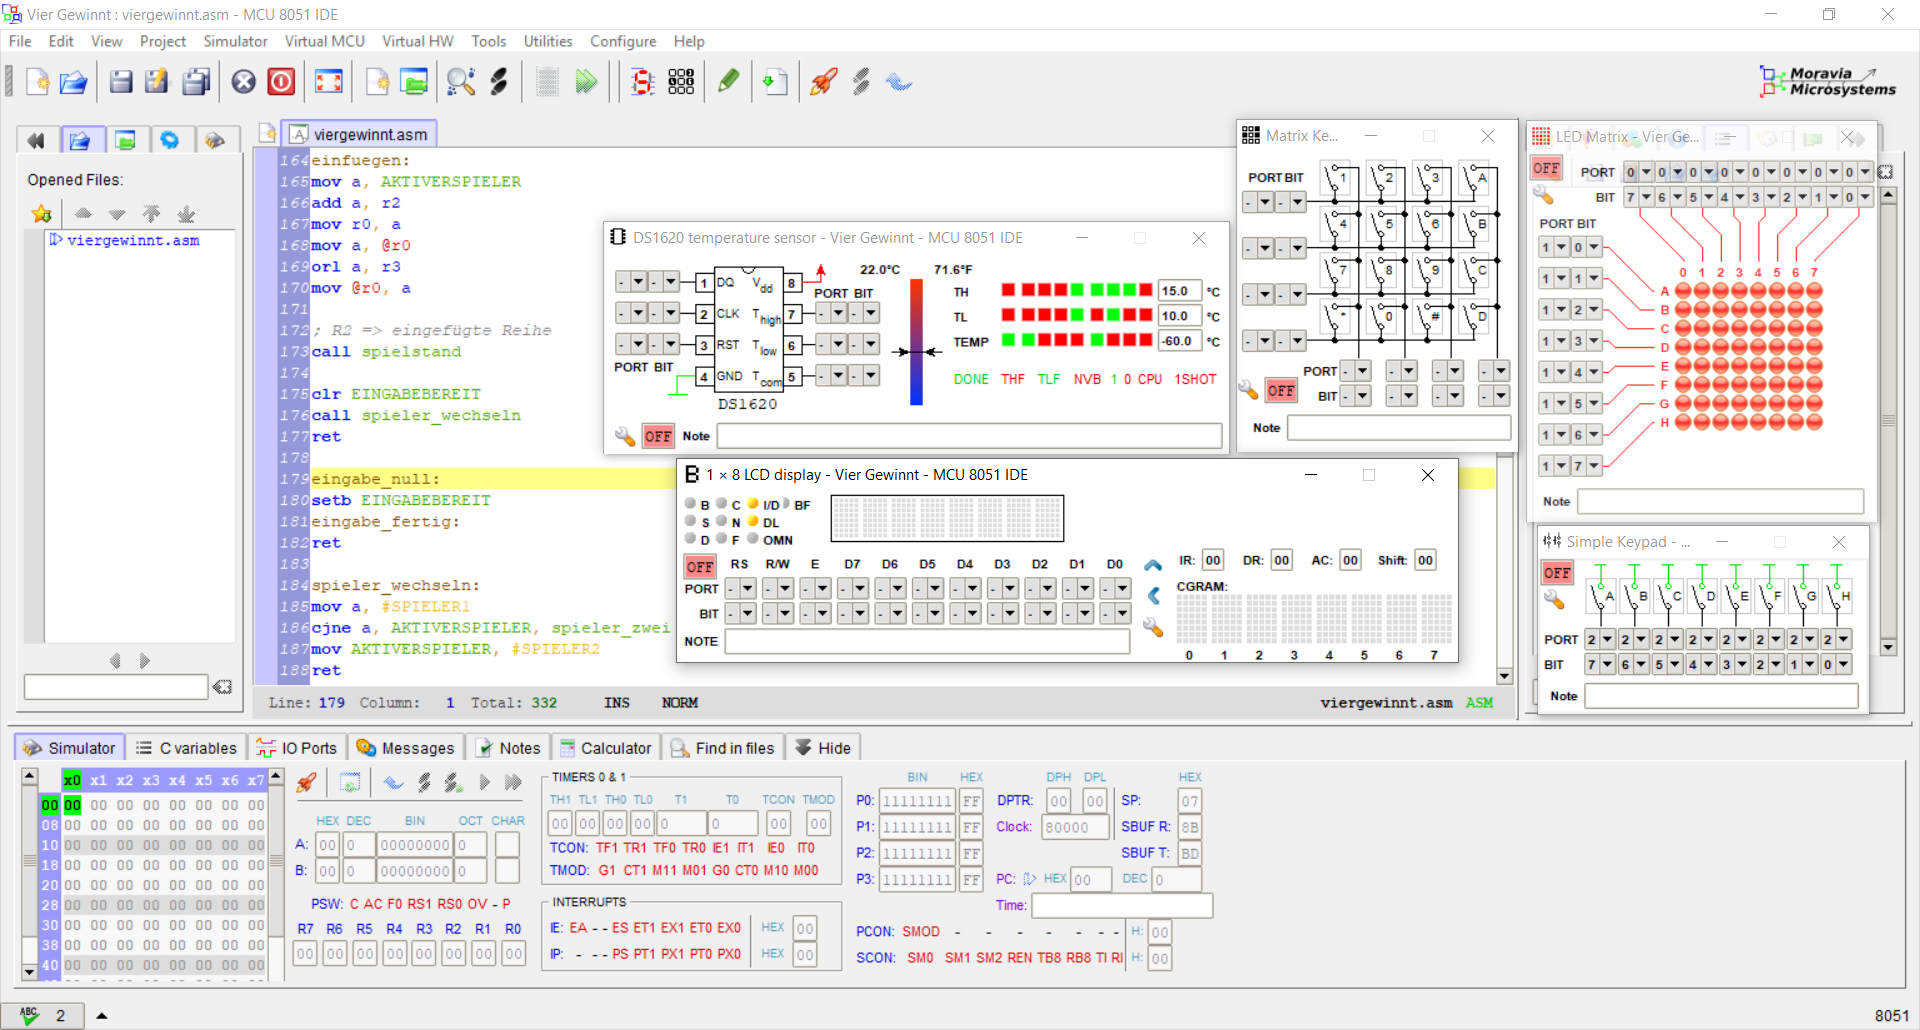
\includegraphics[width=.8\textwidth]{ide.png}
	\caption{MCU-8051 IDE}
	\label{img:grafik-ide}
\end{figure}

Unterteilt wird die IDE in vier verschiedene Bereiche. Mittig befindet sich der eingebaute Texteditor mit zusätzlichem Syntaxhighlighting, -validierung und -autocompleting - In diesem kann in C und Assembler programmiert werden. Links und rechts daneben befindet sich die Projektübersicht und einem Panel zum Debuggen. Darunter die Anzeige für den Speicher, Akkumulator und dem Register des Prozessors. Diese beinhaltet darüber hinaus noch den Timer und die Ports für eine externe Kommunikation.
\FloatBarrier
\chapter{Konzept}

Entwickelt werden soll ein 4-Gewinnt Spiel für zwei Spieler.
Die Ausgabe soll auf einer $8 \cdot 8$ LED-Matrix erfolgen.
Die Eingabe wird durch 8 Schalter ermöglicht.

\section{Analyse}

% TODO: Mehr Analysieren
Da die Entwicklungsumgebung keine mehrfarbige LED-Matrix bereitstellt, werden die Steine des zweiten Spielers durch Blinken von den Steinen des ersten Spielers unterschieden.

\section{Programmentwurf}

% TODO: Irgendwo "eingabebereit" erklären
Der Programmfluss, wie er in \autoref{fig:programmfluss} dargestellt ist, beschreibt den Ablauf des Programms.\\
Nach dem Start des Simulators beginnt die Initialisierung des Programms - der benötigte Speicher wird zurückgesetzt, Spieler 1 als aktiver Spieler ausgewählt und der Timer gestartet. Danach beginnt die Hauptschleife.\\
In ihr wird wiederholt abgefragt, ob aktuell eine Eingabe getätigt werden kann -- also, ob das Keypad vollständig auf false gestellt wurde.
Ist dies möglich prüft eine Schleife auf eine Eingabe durch den aktiven Spieler.
Wurde diese ausgeführt, wird anhand des Zuges überprüft, ob der Spieler es geschafft hat 4 Steine nebeneinander zu setzen.
Ist dies der Fall, hat er gewonnen - andernfalls kommt es zum Spielerwechsel und die Hauptschleife beginnt von Neuem.
Sobald ein Spieler gewonnen hat, wird die Spielerzahl des Siegers angezeigt.
Es besteht die Möglichkeit, ein neues Spiel zu beginnen, indem auf dem Keypad der erste und letzte Taster betätigt werden.
Dann wird der Spieler gewechselt -- also fängt der Verlierer an -- und das Spiel startet erneut.

\begin{figure}
	\centering
  \begin{tikzpicture}[node distance=1.5cm]
    \node (start) [startstop] {Start};
    \node (init) [process, below of=start] {Initialisierung};
    \node (mainloop) [process, below of=init] {Eingabepad auslesen};
    \node (readyforinput) [decision, below of=mainloop, yshift=-1.0cm] {Eingabe zurückgesetzt?};
    \node (getinput) [process, below of=readyforinput, yshift=-1.0cm] {Eingabepad auslesen};
    \node (checkplayerdecision) [decision, below of=getinput, yshift=-1.0cm] {Eingabe gesetzt?};
    \node (checkturn) [process, below of=checkplayerdecision, yshift=-1.0cm] {Eingabe auswerten};
    \node (checkwin) [decision, below of=checkturn, yshift=-1cm] {Gewonnen?};
    \node (switchplayers) [process, right of=checkwin, xshift=5cm] {Spieler wechseln};
    \node (end) [startstop, below of=checkwin, yshift=-1cm] {Spielende};

    \draw [arrow] (start) -- (init);
    \draw [arrow] (init) -- (mainloop);
    \draw [arrow] (mainloop) -- (readyforinput);
    \draw [arrow] (readyforinput) -- node[anchor=west] {ja} (getinput);
    \draw [arrow] (readyforinput) -- node[anchor=south] {nein} (readyforinput-|switchplayers.west) |- ([yshift=8pt]mainloop.south east);
    \draw [arrow] (getinput) -- (checkplayerdecision);
    \draw [arrow] (checkplayerdecision) -- node[anchor=south] {nein} (checkplayerdecision-|switchplayers.west) |- ([yshift=8pt]getinput.south east);
    \draw [arrow] (checkplayerdecision) -- node[anchor=west] {ja} (checkturn);
    \draw [arrow] (checkturn) -- (checkwin);
    \draw [arrow] (checkwin) -- node[anchor=south] {nein} (switchplayers);
    \draw [arrow] (checkwin) -- node[anchor=west] {ja} (end);
    \draw [arrow] (switchplayers) |- ([yshift=-8pt]mainloop.north east);
    \draw [arrow] (end) -- node[anchor=south] {Reset} (end -| switchplayers.south) -- (switchplayers.south);
  \end{tikzpicture}

  \caption{Programmfluss des Spieles}
	\label{fig:programmfluss}
\end{figure}

Zusätzlich zu dieser Hauptschleife wird über ein Timerinterrupt regelmäßig eine Routine ausgeführt, welche das aktuelle Spielbrett ausgibt. Dabei werden die vom ersten Spieler gesetzten Steine auf der LED-Matrix durchgängig beleuchtet, während die Steine des zweiten Spielers blinken.

\begin{highlight}[Hinweis]
  Die Wiederholrate, mit welcher die LED-Matrix aktualisiert wird ist zu groß, um den Blinkeffekt sehen zu können. Sie musste allerdings für die Entwicklung im Simulator so stark erhöht werden, da der Simulator deutlich langsamer als die tatsächliche Hardware ist.
\end{highlight}

\FloatBarrier
\chapter{Implementierung}
Für Vier-Gewinnt kommen folgende Funktionen zum Einsatz:
\begin{itemize}	
	\item Port 0 bis 2
	\item Timer
\end{itemize}

Im ersten Schritt haben wir die Ein- und Ausgabemöglichkeit festgelegt. Als Ausgabe kommt eine LED Matrix, wie in \autoref{img:grafik-ledmatrix} zu sehen ist zum Einsatz, dessen Horizontale über den Port 0 und Vertikale über den Port 1 angesteuert werden. Auf der Matrix werden die Steine der Spieler durch einzelne LEDs angezeigt.
Um zwischen den Steinen beider Spieler unterscheiden zu können, werden die des zweiten Spielers nur bei jeder zweiten Ausgabe angezeigt, sodass diese blinken.


\begin{figure}
	\centering
	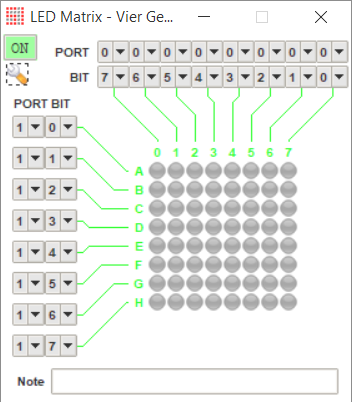
\includegraphics[width=10cm]{ledmatrix.png}
	\caption{LED Matrix - Ausgabewerk}
	\label{img:grafik-ledmatrix}
\end{figure}

Für die Festlegung, welchen Zug der Spieler getätigt bzw. wo dieser einen Stein gesetzt hat kommt ein Keypad, wie es in \autoref{img:grafik-keypad} zu sehen ist zum Einsatz.
Dieses ist mit Port 2 verbunden. Wird ein Schalter betätigt wird der jeweilige Pin mit dem Massepotential verbunden, also auf \enquote{low} gesetzt.

\begin{figure}
	\centering
	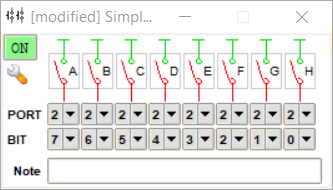
\includegraphics[width=10cm]{keypad.png}
	\caption{Keypad - Eingabewerk}
	\label{img:grafik-keypad}
\end{figure}

Wenn das Spiel beginnt, werden zunächst alle Ports initialisiert, also Port 0 und Port 1 auf \enquote{low} gesetzt, um die Ausgabe zu löschen.
Danach wird der Timer konfiguriert.
Direkt im Anschluss springt der Mikrocomputer in eine Dauerschleife, in welcher er ständig abfragt, ob eine Eingabe getätigt wurde.
Dies ist der Fall, wenn an Port 2 nicht mehr alle Bits auf \enquote{high} gesetzt sind. 
Ausgewertet wird dies, indem zunächst der Wert von Port 2 in den Akkumulator geschrieben wird und anschließend invertiert wird. Sollte nun eine Null im Akkumulator vorliegen, wurde keine Eingabe getätigt.
Andernfalls wird die Eingabe nun bearbeitet, indem berechnet wird, in welcher Zeile der durch den Schalter ausgewählten Spalte der Stein platziert werden muss. Dafür werden alle Zeilen von unten nach oben so lange durchlaufen, bis die aktuelle Zeile eine leere Zelle in der passenden Spalte hat. Sollte die oberste Spalte erreicht werden, ohne dass ein Stein platziert wurde, gilt dieser Zug als \enquote{verloren} und der nächste Spieler ist an der Reihe.

Wurde ein Stein platziert, wird nun ausgewertet, ob der aktuelle Spieler das Spiel gewonnen hat. Dafür werden alle Zeilen von unten nach oben mit den möglichen Steinkombinationen verglichen. Dies geschieht, indem die Zeile mit einem \enquote{gewinnenden} Muster und-verknüpft wird. Entspricht der Zeilenwert nun einer Zahl, welche vier gesetzte Bits hat (15, 30, 60, 120, 240), so hat der aktuelle Spieler gewonnen.
Falls auf diese Weise keine gewinnende Kombination gefunden werden konnte, wird der Spielstand nun Spaltenweise überprüft. Dafür werden immer vier übereinander liegende Zeilen und-verknüpft. Erhält man bei der Verknüpfung ein Ergebnis ungleich Null, so bedeutet dies, das vier Steine übereinander liegen und der aktuelle Spieler hat gewonnen.

Wurde kein Gewinn festgestellt, wird der aktuelle Spieler gewechselt und es wird so lange gewartet, bis alle Knöpfe des Keypads deaktiviert wurden. Dadurch werden versehentliche Eingaben verhindert. 
Ist das Keypad zurück gesetzt worden, kann der nächste Spieler eine Eingabe treffen und die Schleife läuft von vorne ab.

Parallel zur Hauptschleife läuft ein Timer, welcher in definierten Zeitabständen einen Interrupt auslöst.
Dieser Interrupt ist für das Ausgeben des aktuellen Spielstandes auf der LED-Matrix verantwortlich. 
Da der Spielstand für jeden Spieler in 8 Bytes gespeichert ist, ist die Ausgabe sehr simpel. Für jede Zeile werden folgende Schritte ausgeführt:
\begin{itemize}
	\item Kopiere die Bitmaske, welche angibt, ob Spieler 2 ausgegeben werden soll in den Akkumulator (0x00 oder 0xFF)
	\item Und-verknüpfe die Zeile (das Byte) von Spieler 2 mit dem Akkumulator
	\item Oder-verknüpfe die Zeile (das Byte) von Spieler 1 mit dem Akkumulator
	\item Kopiere den Akkumulatorinhalt in Port 0
	\item Setze das Bit der entsprechenden Zeile in Port 1 auf \enquote{high}
	\item Setze das Bit der entsprechenden Zeile in Port 1 auf \enquote{low}
\end{itemize}

Falls ein Spieler gewonnen hat, wird dies signalisiert, indem der Spielstand von Spieler 1 geleert wird und in den Spielstand von Spieler 2 entweder eine Eins oder eine Zwei (entsprechende Muster auf der Matrix) geschrieben werden, je nach dem welcher Spieler gewonnen hat.
Dies sorgt dafür, dass die Spielerzahl des gewinnenden Spielers auf der Matrix blinkt.
Sobald das Spielstand durch die Eingabe der Zahl 129 (erster und letzter Schalter) auf dem Keypad zurückgesetzt wird, fängt das Spiel erneut an.


\FloatBarrier
\chapter{Zusammenfassung}

Insgesamt ist ein spielbares Vier-Gewinnt-Spiel entstanden, welches den Gewinner ausgeben und, wenn gewollt nach erfolgreichem Spielende, neugetartet werden kann.
Leider war es aus zeitlichen Gründen nicht möglich, eine Abfrage für vier diagonal liegende Steine zu programmieren, sodass es relativ schwierig ist in einem Spiel gegen einen anderen Spieler zu gewinnen.
Man muss dazu sagen, dass die Simulatorgeschwindigkeit sich zudem leider auch negativ auf das sonst so packende Spielerlebnis auswirkt, da es relativ lange dauert, bis eine Eingabe sichtbar wird.\\
Nichtsdestotrotz war es uns dennoch durch dieses Projekt möglich, uns mit dem Thema der systemnahen und somit hardwarenahen Programmierung näher auseinanderzusetzen. Wir konnten fernab der gewohnten höhersprachigen Programmiersprachen ein Blick hinter die oft simpel erscheinenden Abläufe eines Programms und die arbeitsweise eines Computers werfen, wodruch das ein oder andere Verständnis vertieft und verbessert werden konnte.


\end{document}